\section{Continuous-Time Dynamics}

\subsection{Most general/generic for smooth system:}

\begin{center}
    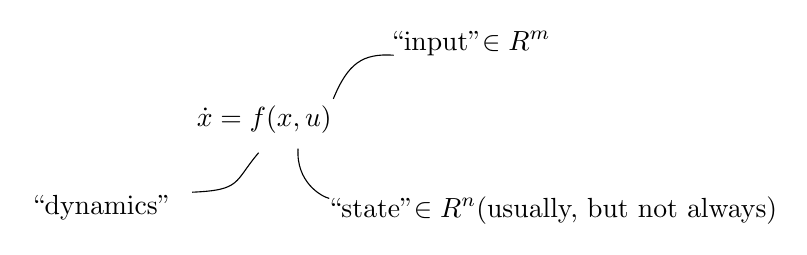
\begin{tikzpicture}[x=0.75pt,y=0.75pt,yscale=-1,xscale=1]
        \draw    (236,169) .. controls (260,168) and (256,164) .. (268,150) ;
        \draw [shift={(270,148)}, rotate = 133] [line width=0.08]  [draw opacity=0] (5,-2) -- (0,0) -- (5,2) -- cycle    ;
        \draw    (302,172) .. controls (298,171) and (286,164) .. (287,148) ;
        \draw [shift={(287,145)}, rotate = 99] [line width=0.08]  [draw opacity=0] (5,-2) -- (0,0) -- (5,2) -- cycle    ;
        \draw    (333,103) .. controls (318,102) and (311,107) .. (304,124) ;
        \draw [shift={(303,127)}, rotate = 292][line width=0.08]  [draw opacity=0] (5,-2) -- (0,0) -- (5,2) -- cycle    ;
        \draw (237,126) node [anchor=north west][inner sep=0.75pt]    {$\dot{x} =f( x,u)$};
        \draw (157,169) node [anchor=north west][inner sep=0.75pt]   [align=left] {``dynamics''};
        \draw (300,170) node [anchor=north west][inner sep=0.75pt]   [align=left] {``state''$\displaystyle \in \mathbb{R}^{n}$(usually, but not always)};
        \draw (330,90) node [anchor=north west][inner sep=0.75pt]   [align=left] {``input''$\displaystyle \in \mathbb{R}^{m}$};
    \end{tikzpicture}
\end{center}

- For a mechanical system (i.e. robotics system):

\begin{center}
    \begin{tikzpicture}[x=0.75pt,y=0.75pt,yscale=-1,xscale=1]
        \draw    (225,39) .. controls (226,27) and (233,21) .. (242,20) ;
        \draw [shift={(245,20)}, rotate = 180] [line width=0.08]  [draw opacity=0] (5,-2) -- (0,0) -- (5,2) -- cycle    ;
        \draw    (226,86) .. controls (230,94) and (236,99) .. (246,100) ;
        \draw [shift={(249,100)}, rotate = 180] [line width=0.08] [draw opacity=0] (5,-2) -- (0,0) -- (5,2) -- cycle;
        \draw (178,38) node [anchor=north west][inner sep=0.75pt]    {$x=\left[\begin{aligned}
                        q \\
                        v
                    \end{aligned}\right]$};
        \draw (251,9) node [anchor=north west][inner sep=0.75pt]   [align=left] {``configuration'' (not always a vector)};
        \draw (250,90) node [anchor=north west][inner sep=0.75pt]   [align=left] {``velocity''};
    \end{tikzpicture}
\end{center}

其中，$q$是系统的configuration，$v$是系统速度。$q$所张成的空间叫做configuration space(位形空间)，整个state space是由$q$和$v$一起构成的流形（manifold）。这个系统描述只有在smooth的时候才是成立的，在某些时候，如四足点着地了，则方程不成立。

同时，$q$并不一定是$\mathbb{R}^{n}$，但是$v$一定是。比如对于单摆系统来说，$q$是单摆的角度，是属于$-\pi$到$\pi$的，因此它所张成的空间是一个圆（因为对于单摆系统来说，转满$\pi$之后则单摆会到的又是$-\pi$的空间了，因此这是一个自己包着自己的compact manifold）。但是对于$v$来说，它的范围是负无穷到正无穷，因此是属于实数空间的。两者一起构成的state space因此是一个圆柱流形。二阶倒立摆的configuration space是一个圆环流形（torus）。

- Example: pendulum

\begin{center}
    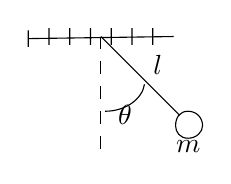
\begin{tikzpicture}[x=0.75pt,y=0.75pt,yscale=-1,xscale=1]
        \draw    (347,16) -- (277,17) (337,20) -- (337,12)(327,20) -- (327,12)(317,20) -- (317,12)(307,20) -- (307,12)(297,20) -- (297,12)(287,20) -- (287,12)(277,21) -- (277,13) ;
        \draw    (312,16) -- (350,54) ;
        \draw  [dash pattern={on 4.5pt off 4.5pt}]  (312,16) -- (312,73) ;
        \draw   (348,59) .. controls (348,55) and (350,52) .. (354,52) .. controls (358,52) and (361,55) .. (361,59) .. controls (361,62) and (358,65) .. (354,65) .. controls (350,65) and (348,62) .. (348,59) -- cycle ;
        \draw  [draw opacity=0] (333,39) .. controls (332,46) and (324,52) .. (314,52) .. controls (314,52) and (314,52) .. (314,52) -- (314,37) -- cycle ; \draw   (333,39) .. controls (332,46) and (324,52) .. (314,52) .. controls (314,52) and (314,52) .. (314,52) ;
        \draw (347,65) node [anchor=north west][inner sep=0.75pt]    {$m$};
        \draw (319,48) node [anchor=north west][inner sep=0.75pt]    {$\theta $};
        \draw (336,24) node [anchor=north west][inner sep=0.75pt]    {$l$};
    \end{tikzpicture}
\end{center}

dynamics equation:

\begin{equation}
    ml^{2}\ddot{\theta } +mgl\sin \theta =\tau
\end{equation}

let $q=\theta,v=\dot\theta$, we get
\begin{equation}
    x=\begin{bmatrix}
        \theta \\
        \dot{\theta }
    \end{bmatrix} \Rightarrow \dot{x} =\begin{bmatrix}
        \dot{\theta } \\
        \ddot{\theta }
    \end{bmatrix} =\underset{f(x,u)}{\underbrace{\begin{bmatrix}
                \dot{\theta } \\
                -\frac{g}{l}\sin \theta +\frac{1}{ml^{2}} u
            \end{bmatrix}}}
\end{equation}

Note that $q\in\mathbb{S}^1$, topology of a circle, $x\in\mathbb{S}^1\times\mathbb{R}$, topology of a cylinder.

\subsection{Control-Affine Systems}

\begin{center}
    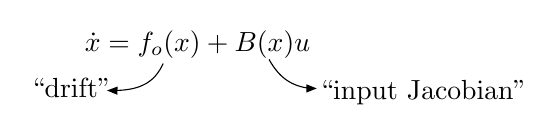
\begin{tikzpicture}[x=0.75pt,y=0.75pt,yscale=-1,xscale=1]
        \draw    (250,26) .. controls (246,35) and (239,39) .. (226,39) ;
        \draw [shift={(223,39)}, rotate = 1] [fill={rgb, 255:red, 0; green, 0; blue, 0 }  ][line width=0.08]  [draw opacity=0] (5,-2) -- (0,0) -- (5,2) -- cycle    ;
        \draw    (301,24) .. controls (306,33) and (312,37) .. (321,38) ;
        \draw [shift={(324,38)}, rotate = 180] [fill={rgb, 255:red, 0; green, 0; blue, 0 }  ][line width=0.08]  [draw opacity=0] (5,-2) -- (0,0) -- (5,2) -- cycle    ;
        \draw (211,9) node [anchor=north west][inner sep=0.75pt]    {$\dot{x} =f_{o}( x) +B( x) u$};
        \draw (185,32) node [anchor=north west][inner sep=0.75pt]   [align=left] {``drift''};
        \draw (324,33) node [anchor=north west][inner sep=0.75pt]   [align=left] {``input Jacobian''};
    \end{tikzpicture}
\end{center}

- most systems can be put in this form

- pendulum:

\begin{equation}
    f_{o}( x) =\begin{bmatrix}
        \dot{\theta } \\
        -\frac{g}{l}\sin \theta
    \end{bmatrix} ,B( x) =\begin{bmatrix}
        0 \\
        \frac{1}{ml^{2}}
    \end{bmatrix}
\end{equation}

如果系统存在一些$u$和$x$的复杂耦合关系使系统无法写成这种标准形式，仍然可以通过一些数学上的trick，通过引入新的状态$\tilde{x}$，这个$\tilde{x}$中包含有原本的$u$和$x$中的耦合部分，则可以变换成这种控制仿射系统。

\subsection{Manipulator Dynamics}

\begin{center}
    
\begin{tikzpicture}[x=0.75pt,y=0.75pt,yscale=-1,xscale=1]
        \draw    (234,26) .. controls (230,35) and (223,39) .. (210,39) ;
        \draw [shift={(207,39)}, rotate = 1] [fill={rgb, 255:red, 0; green, 0; blue, 0 }  ][line width=0.08]  [draw opacity=0] (5,-2) -- (0,0) -- (5,2) -- cycle    ;
        \draw    (284,24) -- (283,35) ;
        \draw [shift={(283,38)}, rotate = 271] [fill={rgb, 255:red, 0; green, 0; blue, 0 }  ][line width=0.08]  [draw opacity=0] (5,-2) -- (0,0) -- (5,2) -- cycle    ;
        \draw    (347,28) .. controls (351,36) and (357,41) .. (367,42) ;
        \draw [shift={(370,42)}, rotate = 180] [fill={rgb, 255:red, 0; green, 0; blue, 0 }  ][line width=0.08]  [draw opacity=0] (5,-2) -- (0,0) -- (5,2) -- cycle    ;
        \draw    (392,19) -- (407,19) ;
        \draw [shift={(410,19)}, rotate = 181] [fill={rgb, 255:red, 0; green, 0; blue, 0 }  ][line width=0.08]  [draw opacity=0] (5,-2) -- (0,0) -- (5,2) -- cycle    ;
        \draw (211,9) node [anchor=north west][inner sep=0.75pt]    {$M( q)\dot{v} +C( q,v) =B( q) u+F$};
        \draw (243,39) node [anchor=north west][inner sep=0.75pt]   [align=center] {``Dynamic Bias''\\(Coriolis+Gravity)};
        \draw (367,34) node [anchor=north west][inner sep=0.75pt]   [align=left] {``Input Jacobian''};
        \draw (412,12) node [anchor=north west][inner sep=0.75pt]   [align=left] {``External Forces''};
        \draw (109,30) node [anchor=north west][inner sep=0.75pt]   [align=left] {``Mass Matrix''};
    \end{tikzpicture}
\end{center}

Just to be cautious that $v$ is not always equal to $\dot q$, but satisfying a certain relationship (Velocity kinematics):

\begin{equation}
    \dot q = G(q) v
\end{equation}

the dynamics can be rewritten as

\begin{equation}
    \dot{x} =f( x,u) =\begin{bmatrix}
        G( q) v \\
        M( q)^{-1}( B( q) u-C)
    \end{bmatrix}
\end{equation}

- Pendulum

\begin{equation}
    M( q) =ml^{2} ,C( q,v) =mgl\sin \theta , B=I, G=I
\end{equation}

- All mechanical systems can be written like this. 机器人动力学建模的两种方法，通过牛顿欧拉和拉格朗日的方法都可以，殊途同归

- This is just a way of re-writing the Euler-Lagrange equation for:

\begin{center}
    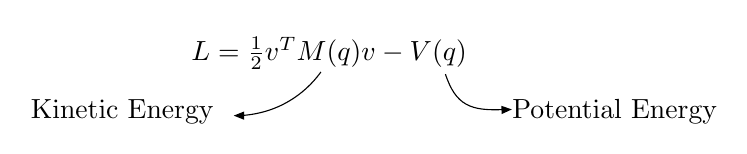
\begin{tikzpicture}[x=0.75pt,y=0.75pt,yscale=-1,xscale=1]
        \draw    (282,67) .. controls (300,66) and (313,57) .. (321,46) ;
        \draw [shift={(279,67)}, rotate = 0] [fill={rgb, 255:red, 0; green, 0; blue, 0 }  ][line width=0.08]  [draw opacity=0] (5,-2) -- (0,0) -- (5,2) -- cycle    ;
        \draw    (410,64) .. controls (393,65) and (386,62) .. (381,47) ;
        \draw [shift={(413,64)}, rotate = 177] [fill={rgb, 255:red, 0; green, 0; blue, 0 }  ][line width=0.08]  [draw opacity=0] (5,-2) -- (0,0) -- (5,2) -- cycle    ;
        \draw (325,37) node    {$L=\frac{1}{2} v^{T} M( q) v-V( q)$};
        \draw (180,58) node [anchor=north west][inner sep=0.75pt]   [align=left] {Kinetic Energy};
        \draw (412,58) node [anchor=north west][inner sep=0.75pt]   [align=left] {Potential Energy};
    \end{tikzpicture}
\end{center}

\subsection{Linear Systems}

\begin{equation}
    \dot x = A(t) x + B(t) u
\end{equation}

- Called ``time invariant'' if $A(t)=A,B(t)=B$

- Called ``time varying'' otherwise

- Super important in control

- We often approximate nonlinear systems with linear ones

\begin{equation}
    \dot{x} =f( x,u) \Rightarrow A=\frac{\partial f}{\partial x} ,B=\frac{\partial f}{\partial u}
\end{equation}

\subsection{Equilibria}

- A point where the system will ``remain at rest'': $\dot{x} =f( x,u) =0$.

- Algebraically, roots of the dynamics.

- Pendulum:

\begin{equation}
    \dot{x} =\begin{bmatrix}
        \dot{\theta } \\
        -\frac{g}{l}\sin \theta
    \end{bmatrix} =\begin{bmatrix}
        0 \\
        0
    \end{bmatrix} \Rightarrow \begin{matrix}
        \dot{\theta } =0 \\
        \theta =0,\pi
    \end{matrix}
\end{equation}

\subsection{First Control Problem}

- Can I move the equilibria?

For example, how to move the pendulum system's equilibria to $\frac{\pi}{2}$, i.e., $\frac{\pi}{2}$ is the root of the equation:
\begin{equation}
    \dot{x} =\begin{bmatrix}
        \dot{\theta } \\
        -\frac{g}{l}\sin \frac{\pi}{2} +\frac{1}{ml^{2}} u
    \end{bmatrix} = 0
\end{equation}

we get $u=mgl$ and $\dot\theta=0$.

- In general, this is a root-finding problem: $f(x^*,u)=0$

\subsection{Stability of Equilibria}

- Stability must be associated with a certain equilibria, or else it is meaningless.

- Definition: What would happen when we stay ``near'' an equilibrium point under perturbations.

- Example: 1-D system

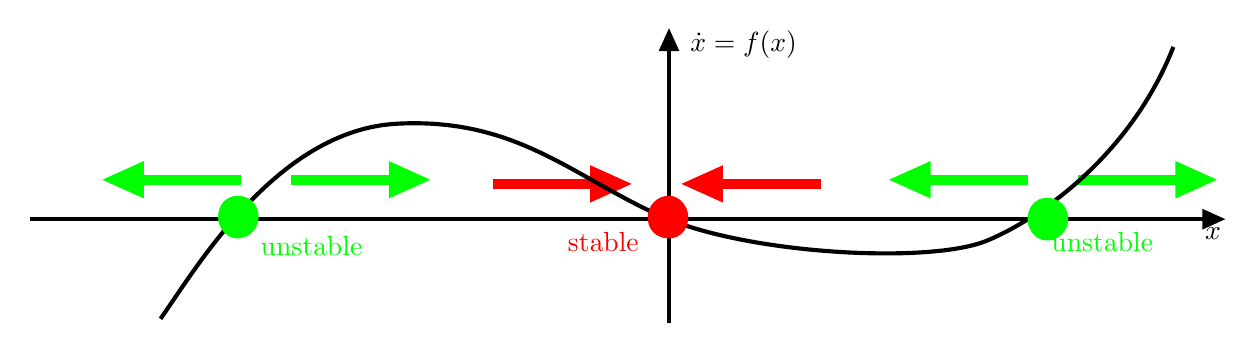
\begin{tikzpicture}[x=0.75pt,y=0.75pt,yscale=-1,xscale=1]
    \draw [color={rgb, 255:red, 0; green, 255; blue, 0 }  ,draw opacity=1 ][line width=3.75]    (103,77) -- (43,77) ;
    \draw [shift={(36,77)}, rotate = 360] [fill={rgb, 255:red, 0; green, 255; blue, 0 }  ,fill opacity=1 ][line width=0.08]  [draw opacity=0] (20,-9) -- (0,0) -- (20,9) -- cycle    ;
    \draw [color={rgb, 255:red, 0; green, 255; blue, 0 }  ,draw opacity=1 ][line width=3.75]    (127,77) -- (187,77) ;
    \draw [shift={(194,77)}, rotate = 180] [fill={rgb, 255:red, 0; green, 255; blue, 0 }  ,fill opacity=1 ][line width=0.08]  [draw opacity=0] (20,-9) -- (0,0) -- (20,9) -- cycle    ;
    \draw [color={rgb, 255:red, 0; green, 255; blue, 0 }  ,draw opacity=1 ][line width=3.75]    (482,77) -- (422,77) ;
    \draw [shift={(415,77)}, rotate = 360] [fill={rgb, 255:red, 0; green, 255; blue, 0 }  ,fill opacity=1 ][line width=0.08]  [draw opacity=0] (20,-9) -- (0,0) -- (20,9) -- cycle    ;
    \draw [color={rgb, 255:red, 0; green, 255; blue, 0 }  ,draw opacity=1 ][line width=3.75]    (506,77) -- (566,77) ;
    \draw [shift={(573,77)}, rotate = 180] [fill={rgb, 255:red, 0; green, 255; blue, 0 }  ,fill opacity=1 ][line width=0.08]  [draw opacity=0] (20,-9) -- (0,0) -- (20,9) -- cycle    ;
    \draw [color={rgb, 255:red, 255; green, 0; blue, 0 }  ,draw opacity=1 ][line width=3.75]    (224,79) -- (284,79) ;
    \draw [shift={(291,79)}, rotate = 180] [fill={rgb, 255:red, 255; green, 0; blue, 0 }  ,fill opacity=1 ][line width=0.08]  [draw opacity=0] (20,-9) -- (0,0) -- (20,9) -- cycle    ;
    \draw [color={rgb, 255:red, 255; green, 0; blue, 0 }  ,draw opacity=1 ][line width=3.75]    (382,79) -- (322,79) ;
    \draw [shift={(315,79)}, rotate = 360] [fill={rgb, 255:red, 255; green, 0; blue, 0 }  ,fill opacity=1 ][line width=0.08]  [draw opacity=0] (20,-9) -- (0,0) -- (20,9) -- cycle    ;
    \draw [line width=1.5]    (1,96) -- (573,96) ;
    \draw [shift={(577,96)}, rotate = 180] [fill={rgb, 255:red, 0; green, 0; blue, 0 }  ][line width=0.08]  [draw opacity=0] (11,-5) -- (0,0) -- (11,5) -- cycle    ;
    \draw [line width=1.5]    (309,8) -- (309,146) ;
    \draw [shift={(309,4)}, rotate = 90] [fill={rgb, 255:red, 0; green, 0; blue, 0 }  ][line width=0.08]  [draw opacity=0] (11,-5) -- (0,0) -- (11,5) -- cycle    ;
    \draw [line width=1.5]    (64,144) .. controls (81,120) and (120,53) .. (178,50) .. controls (235,47) and (262,75) .. (304,94) .. controls (345,113) and (436,118) .. (463,106) .. controls (489,95) and (532,64) .. (552,13) ;
    \draw  [color={rgb, 255:red, 0; green, 255; blue, 0 }  ,draw opacity=1 ][fill={rgb, 255:red, 0; green, 255; blue, 0 }  ,fill opacity=1 ] (92,95) .. controls (92,89) and (96,85) .. (101,85) .. controls (107,85) and (111,89) .. (111,95) .. controls (111,100) and (107,105) .. (101,105) .. controls (96,105) and (92,100) .. (92,95) -- cycle ;
    \draw  [color={rgb, 255:red, 0; green, 255; blue, 0 }  ,draw opacity=1 ][fill={rgb, 255:red, 0; green, 255; blue, 0 }  ,fill opacity=1 ] (482,96) .. controls (482,90) and (486,86) .. (491,86) .. controls (497,86) and (501,90) .. (501,96) .. controls (501,101) and (497,106) .. (491,106) .. controls (486,106) and (482,101) .. (482,96) -- cycle ;
    \draw  [color={rgb, 255:red, 255; green, 0; blue, 0 }  ,draw opacity=1 ][fill={rgb, 255:red, 255; green, 0; blue, 0 }  ,fill opacity=1 ] (299,95) .. controls (299,90) and (303,85) .. (309,85) .. controls (314,85) and (318,90) .. (318,95) .. controls (318,101) and (314,105) .. (309,105) .. controls (303,105) and (299,101) .. (299,95) -- cycle ;
    \draw (318,4) node [anchor=north west][inner sep=0.75pt]    {$\dot{x} =f( x)$};
    \draw (566,99) node [anchor=north west][inner sep=0.75pt]    {$x$};
    \draw (111,103) node [anchor=north west][inner sep=0.75pt]   [align=left] {\textcolor[rgb]{0,1,0}{unstable}};
    \draw (492,101) node [anchor=north west][inner sep=0.75pt]   [align=left] {\textcolor[rgb]{0,1,0}{unstable}};
    \draw (259,101) node [anchor=north west][inner sep=0.75pt]   [align=left] {\textcolor[rgb]{1,0,0}{stable}};
\end{tikzpicture}


As for 1-D system, the criterion is simple: $\frac{\partial f}{\partial x}<0\Rightarrow\text{stable}$ , $\frac{\partial f}{\partial x}>0\Rightarrow\text{unstable}$.

- In higher dimensions

$\frac{\partial f}{\partial x}$ is a Jacobian matrix, take an eigen decomposition:

\begin{align*}
    \text{Re}\left[\text{eig}\left(\frac{\partial f}{\partial x}\right)\right]<0 \Rightarrow \text{stable} \\
    \text{Otherwise} \Rightarrow \text{unstable}
\end{align*}

我们可以通过找到一组坐标线性变换方式（coordinate transformation）,将系统的所有状态转化成独立的，则将$n$维系统转成$n$个独立的子系统。而这一步就是对系统的雅可比矩阵进行特征值分解，分解后每个特征向量对应的特征值则是对应子系统的梯度值。

- Pendulum:

\begin{align*}
    f(x)                                                       & =\begin{bmatrix}
        \dot{\theta } \\
        -\frac{g}{l}\sin \theta
    \end{bmatrix} \Rightarrow
    \frac{\partial f}{\partial x} =
    \begin{bmatrix}
        0                       & 1 \\
        -\frac{g}{l}\cos \theta & 0
    \end{bmatrix}                                                                                                                                                                                    \\
    \left.\frac{\partial f}{\partial x}\right| _{\theta =\pi } & =\begin{bmatrix}
        0           & 1 \\
        \frac{g}{l} & 0
    \end{bmatrix} \Rightarrow \text{eig}\left(\frac{\partial f}{\partial x}\right) =\pm \sqrt{\frac{g}{l}} \Rightarrow \text{unstable} \\
    \left. \frac{\partial f}{\partial x}\right| _{\theta =0}   & =\begin{bmatrix}
        0            & 1 \\
        -\frac{g}{l} & 0
    \end{bmatrix} \Rightarrow \text{eig}\left(\frac{\partial f}{\partial x}\right) =\pm i\sqrt{\frac{g}{l}}
\end{align*}

- Pure imaginary case is called ``marginally stable'': undamped oscillations. 这意味着，假如在平衡点处给一点小扰动，那么单摆在没有空气阻力的情况下将会一直荡下去。

- Add damping (e.g. $u=-k_d\dot\theta$) results in strictly negative real part.

Lecture 1和2的主线基本上是从一个最简单的单摆系统开始，介绍现代控制理论中的一些基本知识，与本科阶段我上过的课的内容差异不大。本节先介绍了连续系统的不同状态方程以及如何判断系统平衡点处的稳定性。平衡点的概念对于一个非线性系统的控制来说是比较重要的，因为我们可以在平衡点处对非线性系统进行线性化后再利用成熟的线性控制理论来求解复杂的非线性控制问题。

\subsection{Introduction to Julia}

Coding...